\documentclass[11pt,a4paper]{ctexart}
\usepackage[a4paper,margin=1.55cm]{geometry}
\usepackage{fontspec}
\usepackage{xeCJK}
\usepackage{graphicx}
\usepackage{booktabs}
\usepackage{tabularx}
\usepackage{array}
\usepackage{xcolor}
\usepackage{titlesec}
\usepackage{enumitem}
\usepackage{amsmath}
\usepackage{tcolorbox}
\tcbuselibrary{skins}
\usepackage{fancyhdr}
\usepackage{lastpage}
\usepackage{hyperref}
\usepackage{float}
\usepackage{setspace}
\usepackage{caption}

\setmainfont{Times New Roman}
\setsansfont{Arial}
\setmonofont{Consolas}
\setCJKmainfont[
  Path=fonts/,
  BoldFont=NotoSerifCJKsc-Bold.otf
]{NotoSerifCJKsc-Regular.otf}
\setCJKsansfont[
  Path=fonts/,
  BoldFont=NotoSansCJKsc-Bold.otf
]{NotoSansCJKsc-Regular.otf}
\setCJKmonofont[
  Path=fonts/
]{NotoSansMonoCJKsc-Regular.otf}
\xeCJKsetup{PunctStyle=kaiming, CJKmath=true}

\hypersetup{colorlinks=true,linkcolor=black,urlcolor=black}
\pagestyle{fancy}
\fancyhf{}
\fancyfoot[R]{\thepage/\pageref{LastPage}}
\renewcommand{\headrulewidth}{0pt}
\renewcommand{\footrulewidth}{0pt}

\definecolor{titleblue}{HTML}{243B53}
\definecolor{accent}{HTML}{A23E48}
\definecolor{softblue}{HTML}{EDF3F8}
\definecolor{softgray}{HTML}{F5F7FA}
\definecolor{linegray}{HTML}{D9E2EC}

\setlength{\parindent}{0pt}
\setlength{\parskip}{4pt}
\setstretch{1.08}
\captionsetup{font=small}

\titleformat{\section}{\large\bfseries\color{titleblue}}{\thesection.}{0.5em}{}
\titleformat{\subsection}{\normalsize\bfseries\color{titleblue}}{\thesubsection}{0.5em}{}
\titlespacing*{\section}{0pt}{8pt}{5pt}
\titlespacing*{\subsection}{0pt}{5pt}{3pt}

\newcommand{\metricbox}[2]{
  \begin{tcolorbox}[
    enhanced,
    colback=softblue,
    colframe=linegray,
    boxrule=0.4pt,
    arc=2mm,
    left=3mm,right=3mm,top=2mm,bottom=2mm,
    width=\linewidth,
    height=1.55cm
  ]
  {\small\color{gray!80!black}#1}\\[2pt]
  {\Large\bfseries\color{titleblue}#2}
  \end{tcolorbox}
}

\begin{document}

\begin{center}
  {\fontsize{18}{21}\selectfont\bfseries\color{titleblue} 宁波怡丰汇商业项目案例研究报告}\\[6pt]
  {\small 工程经济学 Case Study}\\[4pt]
  {\small 姓名与学号：杜楷劼 2025316285 \quad 李博文 2025316286 \quad 王一燚 2025316289}
\end{center}

\vspace{3pt}
\begin{center}
\begin{minipage}[t]{0.47\textwidth}
\metricbox{Recommended Purchase Price}{3.33 亿元}
\end{minipage}\hfill
\begin{minipage}[t]{0.47\textwidth}
\metricbox{Initial Total Investment}{3.64 亿元}
\end{minipage}

\vspace{3pt}

\begin{minipage}[t]{0.47\textwidth}
\metricbox{Terminal Value}{4.42 亿元}
\end{minipage}\hfill
\begin{minipage}[t]{0.47\textwidth}
\metricbox{Target MARR}{12\%}
\end{minipage}
\end{center}

\section{Step 1：建立现金流模型}

\subsection{建模视角与现金流阶段}

本案例从\textbf{投资委员会/买方}视角建立现金流图（Cash Flow Diagram）。按照工程经济学的\textbf{相关现金流}原则，模型只纳入收购决策之后发生、且与项目实施直接相关的现金流；项目历史租金水平仅作为判断经营现状与招商风险的背景，不作为未来现金流输入。研究期以 \texttt{2026-01-01} 为 \textbf{Period 0}，\texttt{2026} 年为题目定义的改造期，\texttt{2027--2029} 年为稳定运营期。题目要求“不考虑折旧”，因此模型直接计算税前现金流（BTCF）与税后现金流（ATCF）。

\begin{table}[H]
  \centering
  \small
  \begin{tabularx}{\textwidth}{>{\bfseries}p{2.3cm} p{2.1cm} p{3.0cm} X}
    \toprule
    现金流阶段 & 时间 & 模型定位 & 计量口径 \\
    \midrule
    项目获取 & 2026-01-01 & Period 0 & 支付收购对价、契税、其他交易费用和开业成本，作为期初投资现金流出。 \\
    改造期 & 2026Q1 & 开业准备阶段 & 尚未产生经营性现金流，发生取得项目后必要的准备与改造支出。 \\
    免租运营期 & 2026Q2 & 开业后租金暂免 & 停车费和物业费计入收入，租金收入为零，O\&M 成本开始发生。 \\
    首年收租期 & 2026Q3--Q4 & 改造期内正式收租 & 租金开始计收，现金流由负压区间转向经营现金流转正。 \\
    稳定运营期 & 2027--2029 & 全年运营阶段 & 出租率按 95\% 估计，全年计量收入、成本、税费和 ATCF。 \\
    项目退出 & 2029-12-31 & 期末残值现金流 & 以 2029 年 ATCF 永续资本化估计退出价值，退出价值不计税。 \\
    \bottomrule
  \end{tabularx}
\end{table}

\subsection{相关现金流与计算口径}

题目 Step 1 要求识别投资成本、租金收入、停车费收入、物业费收入、运营成本、退出价值和税收成本。下表将题目要求转化为现金流模型输入，保证各项现金流在同一研究期、同一投资人视角下计量。

\begin{table}[H]
  \centering
  \small
  \begin{tabularx}{\textwidth}{>{\bfseries}p{2.45cm} X}
    \toprule
    现金流项目 & 计量口径 \\
    \midrule
    投资成本 & Period 0 支付收购对价、3\% 契税、1100 万元其他交易费用和 1000 万元开业成本，作为获取阶段一次性投资成本。 \\
    租金收入 & 按楼层可租面积、日租金、出租率和收租天数计量；2026 年仅收 184 天租金，2027--2029 年按全年收取，2029 年租金增长 3\%。 \\
    停车费收入 & 1005 个车位统一运营，按 3 元/小时、6 小时/天、车位使用率和实际运营天数计入经营收益。 \\
    物业费收入 & 按实际出租面积、10 元/平方米/月计取；免租期租金免收，但物业费照常收取。 \\
    运营成本 & 人事、推广、维修、物管、能耗、行政等 O\&M 成本在 2026 年按 9/12 折算，2027 年起按全年口径并根据费用增长率递推。 \\
    退出价值 & \(TV_{2029}=\text{ATCF}_{2029}/8\%\)，作为 2029 年末终值现金流，退出价值不计税。 \\
    税收成本 & 不考虑折旧时，营业利润直接形成所得税税基，\(\text{Tax}_t=\max(\text{BTCF}_t,0)\times25\%\)。 \\
    \bottomrule
  \end{tabularx}
\end{table}

收入端分为租金、停车费和物业费三类，成本端分为周期性 O\&M 成本和资本性改造支出。记 \(A_i\) 为楼层 \(i\) 的可租面积，\(r_i\) 为日租金，\(D_t\) 为收租天数，\(Occ_t\) 为出租率，\(g_t\) 为租金增长因子，则：
\begin{align*}
\text{Revenue}_t &= \text{Rent}_t+\text{Parking}_t+\text{PropertyFee}_t \\
\text{Rent}_t &= \sum_i A_i r_i D_t Occ_t g_t \\
\text{Parking}_t &= N_p p_h h_d u_t OD_t \\
\text{PropertyFee}_t &= A_{\text{rentable}} Occ_t f_m M_t \\
\text{BTCF}_t &= \text{Revenue}_t-\text{O\&M}_t-\text{CapexReno}_t \\
\text{Tax}_t &= \max(\text{BTCF}_t,0)\times25\%, \qquad
\text{ATCF}_t=\text{BTCF}_t-\text{Tax}_t
\end{align*}

\subsection{年度税后现金流结果}

基准情形下，2026 年由于仅运营 9 个月且包含 3 个月免租期，ATCF 明显低于稳定期；2027 年后出租率提升至 95\%，收入和成本进入全年口径。2028 年按实际年度天数 366 天计算。

\begin{table}[H]
  \centering
  \scriptsize
  \begin{tabularx}{\textwidth}{>{\bfseries}l *{4}{>{\raggedleft\arraybackslash}X}}
    \toprule
    单位：万元 & 2026 & 2027 & 2028 & 2029 \\
    \midrule
    出租率 & 80\% & 95\% & 95\% & 95\% \\
    租金收入 & 2297.87 & 5412.94 & 5427.77 & 5575.33 \\
    停车费收入 & 248.74 & 396.17 & 463.47 & 528.23 \\
    物业费收入 & 450.93 & 713.98 & 713.98 & 713.98 \\
    营业收入合计 & 2997.54 & 6523.09 & 6605.22 & 6817.54 \\
    运营成本合计 & 1527.32 & 2090.39 & 2102.76 & 2105.18 \\
    税前现金流 BTCF & 1470.22 & 4432.70 & 4502.45 & 4712.36 \\
    企业所得税 & 367.55 & 1108.18 & 1125.61 & 1178.09 \\
    税后现金流 ATCF & 1102.66 & 3324.53 & 3376.84 & 3534.27 \\
    \bottomrule
  \end{tabularx}
\end{table}

\begin{figure}[H]
  \centering
  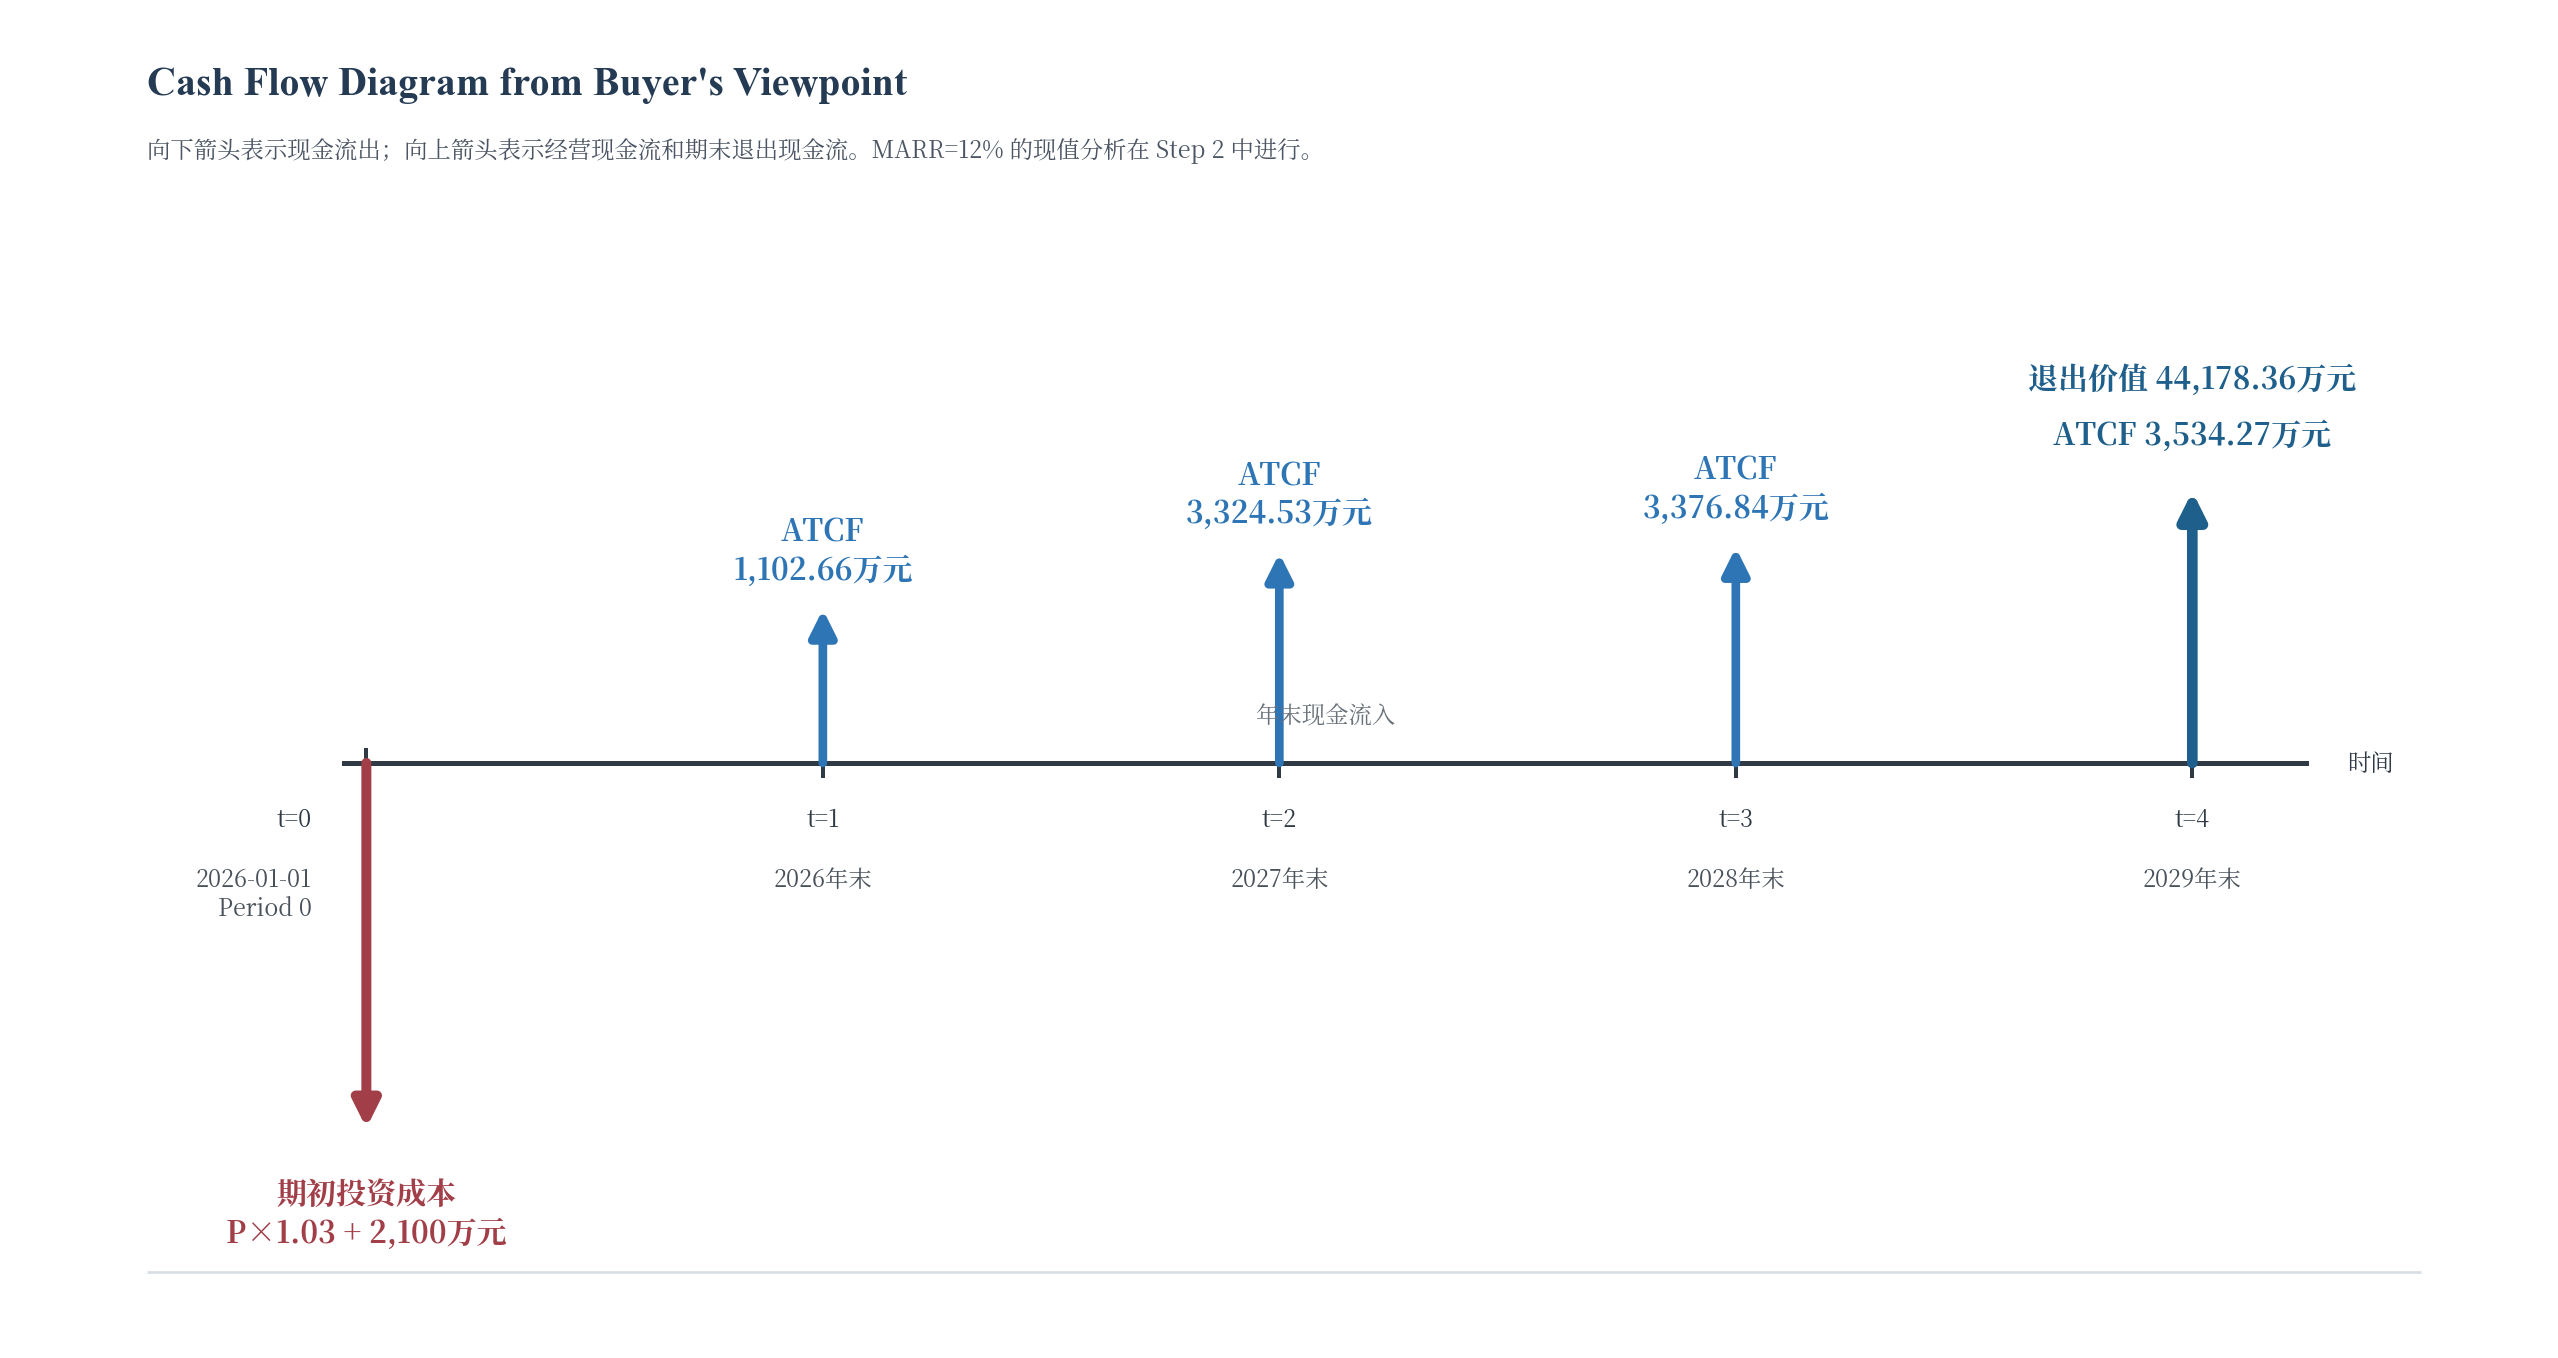
\includegraphics[width=0.98\textwidth]{figures/cash_flow_diagram.png}
  \caption{买方视角下的项目现金流图}
\end{figure}

从收入结构看，\textbf{租金收入}是项目的核心现金流入，2027 年以后稳定在 \textbf{5400--5600 万元}区间；\textbf{物业费}在免租期仍可收取，提供一定防守性；\textbf{停车收入}随车位利用率提高逐年增长。该结构说明，本项目经济可行性的基础不是历史 400 万元租金，而是改造招商后能否形成稳定出租率和持续经营现金流。

\subsection{2026 年季度改善与稳定期差异}

题目要求判断现金流是否逐季度改善。2026 年现金流改善具有明显的阶段性：Q1 尚未营业；Q2 虽已开业但仍处于免租期，收入主要来自停车费和物业费，而人事、物业管理、能耗等 O\&M 成本已经发生；Q3 开始收租后，租金现金流入覆盖固定性运营成本，季度经营现金流转正。

\begin{figure}[H]
  \centering
  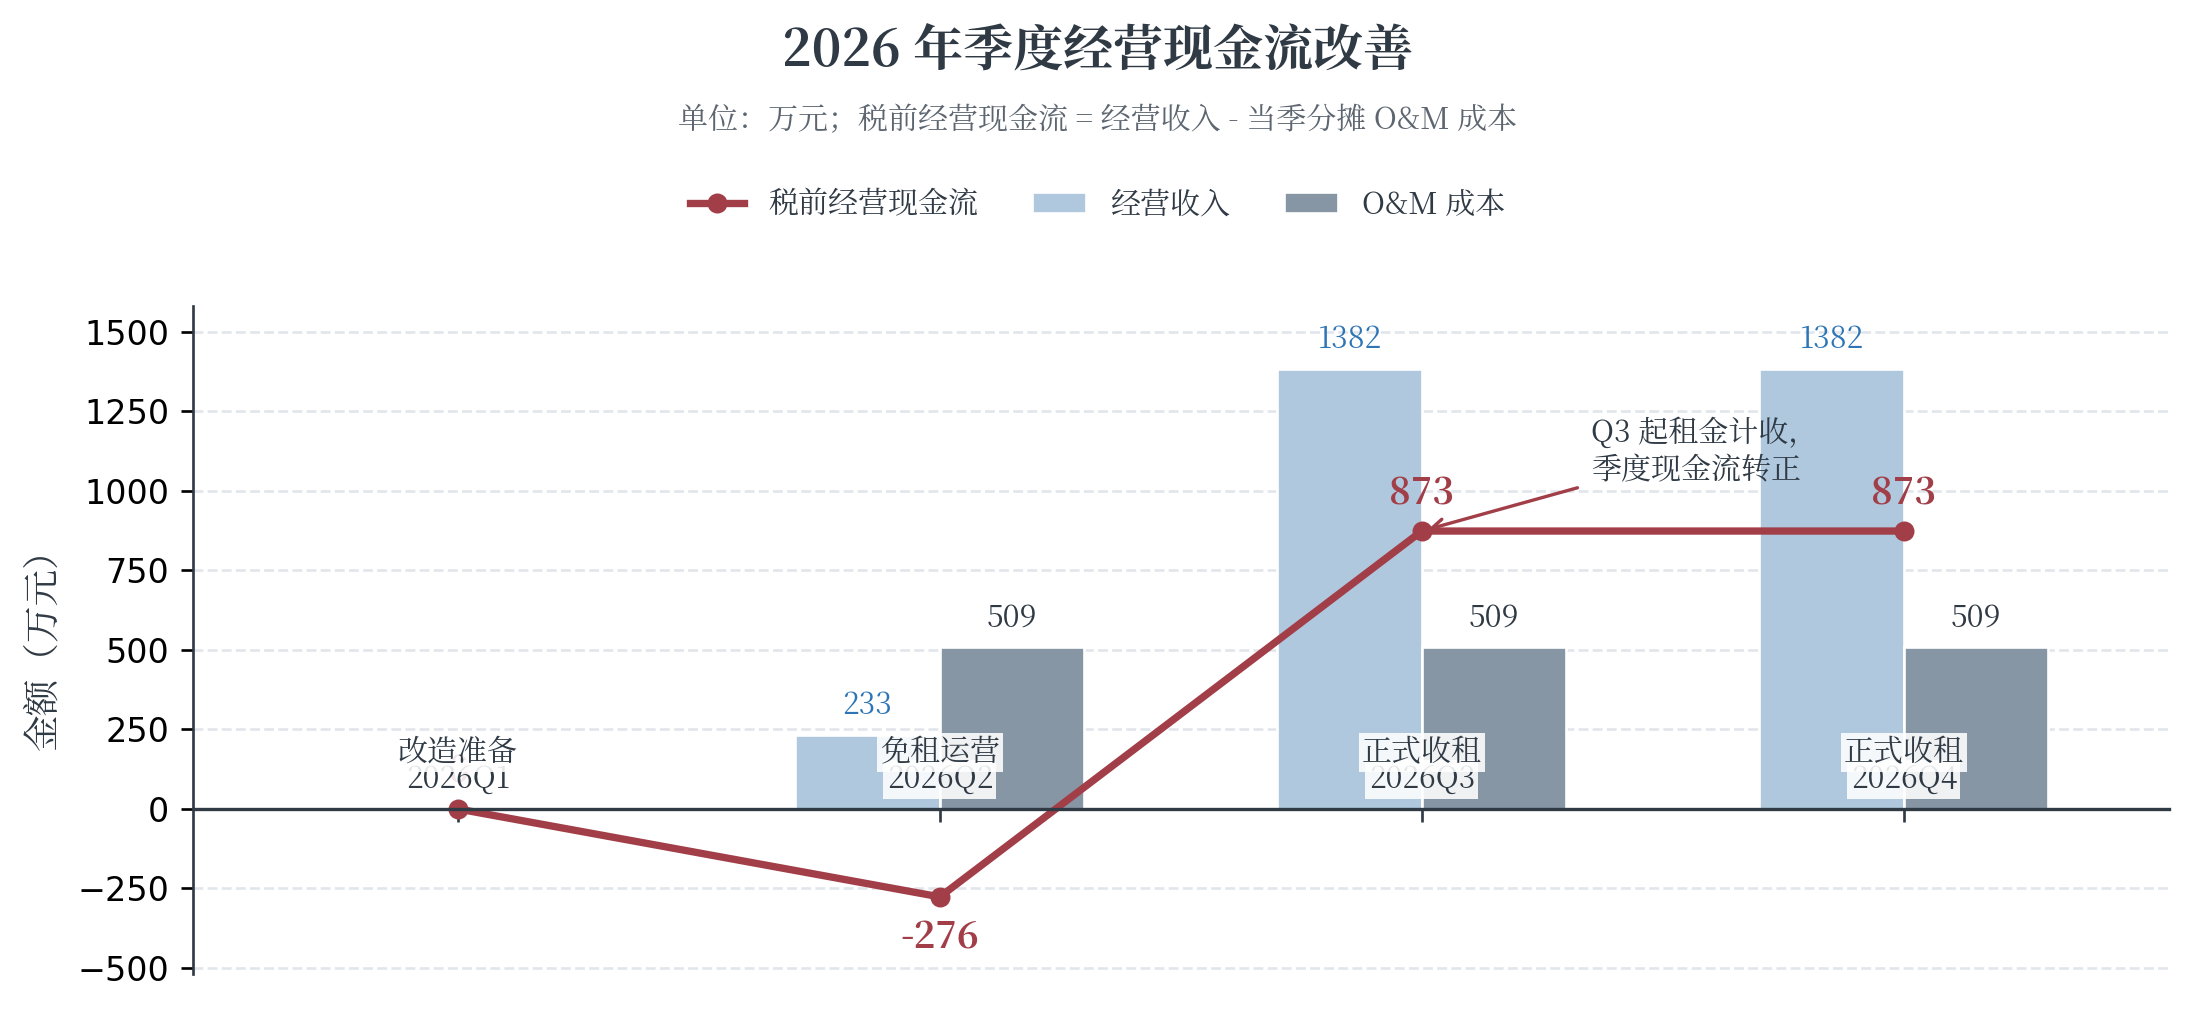
\includegraphics[width=0.94\textwidth]{figures/quarterly_ramp_chart.png}
  \caption{2026 年季度经营现金流改善：免租期后现金流转正}
\end{figure}

改造期与稳定期差异显著：2026 年 ATCF 为 \textbf{1102.66 万元}，仅为 2027 年 \textbf{3324.53 万元}的约 \textbf{33.2\%}；稳定期第一年较改造期增加约 \textbf{2221.87 万元}，增幅约 \textbf{201.5\%}。主要原因是 2026 年只收 6 个月租金、出租率从 80\% 提升至 95\%，且停车使用率从 50\% 逐年提高；同时首年 O\&M 成本具有较强固定成本特征，免租期会放大现金流压力。

\section{Step 2：收购价格估算}

\subsection{投资结论}

基于题目给定假设，在 \texttt{MARR = 12\%}、退出资本化率 \texttt{8\%} 的条件下，本项目的合理收购对价约为 \textbf{3.33 亿元}。对应的初始总投资额约为 \textbf{3.64 亿元}，其中已包含收购对价、\texttt{3\%} 契税、\texttt{1100 万元}其他交易费用及 \texttt{1000 万元}开业成本。

项目在 \texttt{2026} 年处于改造与招商阶段，经营现金流明显低于稳定期；从 \texttt{2027} 年开始，出租率提升至 \texttt{95\%} 后，现金流进入稳定区间。若卖方报价明显高于 \textbf{3.33 亿元}，则项目难以满足 \texttt{12\%} 的最低可接受报酬率要求，因此该价格应视为投资上限而非议价起点。

\begin{figure}[H]
  \centering
  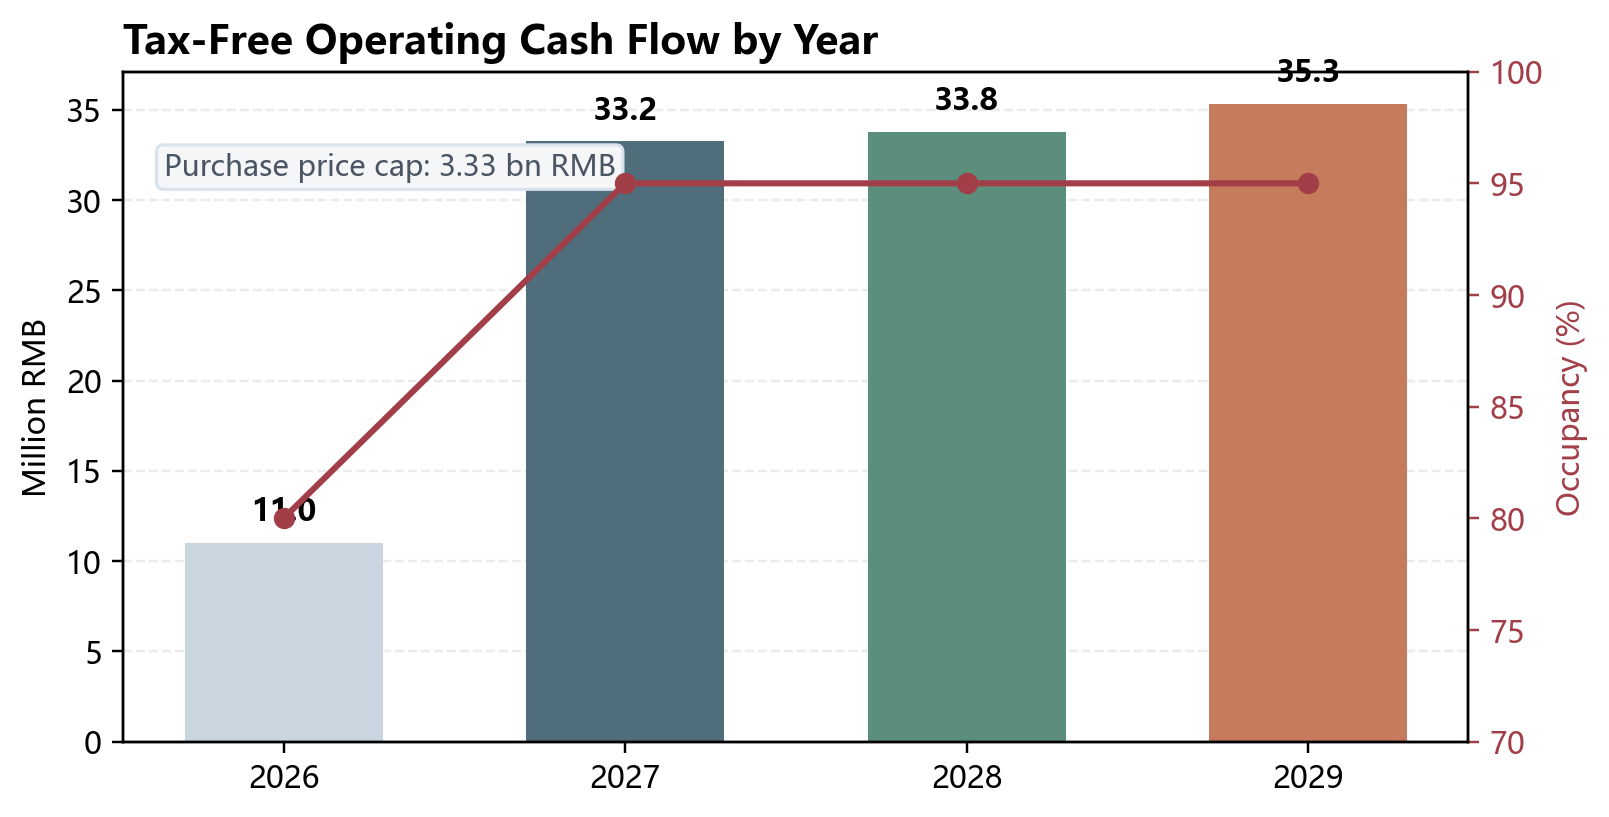
\includegraphics[width=0.94\textwidth]{figures/cash_flow_chart.png}
  \caption{Tax-free operating cash flow and occupancy by year}
\end{figure}

\subsection{成本、税收与估值推导}

合理收购价按工程经济学标准符号应先写为：
\[
P_0=\frac{\sum_{t=2026}^{2029} \text{ATCF}_t(P/F,12\%,N_t)+\text{TV}_{2029}(P/F,12\%,4)-C_{\text{open}}-C_{\text{other}}}{1+\tau}
\]
代入本题参数后，可写成：
\[
\text{Purchase Price}=\frac{\sum_{t=2026}^{2029}\frac{\text{ATCF}_{t}}{(1+12\%)^{t-2025}}+\frac{\text{TV}_{2029}}{(1+12\%)^4}-\text{Opening Cost}-\text{Other Fees}}{1+3\%}
\]
进一步代入计算结果，有：
\[
P_0 \approx 3.33 \text{ 亿元}
\]
其中，\(\tau=3\%\) 为契税税率。由于本题退出价值采用永续资本化而非有限年金，因此这里不直接使用 \((P/A,i,N)\) 因子；但若把稳定经营期截断为有限持有期，也可以用 \((P/A,i,N)\) 对年等额净现金流做近似表示。

成本端方面，\texttt{2026} 年的人事、市场推广、维保维修、物业管理、能耗和行政支出按 9 个月折算；\texttt{2027} 年以后恢复全年口径，并按题目给定的费用增长率递推。与此同时，资本性改造支出按租金收入的 \texttt{2.5\%} 计提，用于反映招商调整和持续改造需求。

税收处理采用单一企业所得税税率 \texttt{25\%}。由于题目明确要求退出价值\textbf{不计税}，因此项目的年度税负只作用于经营期利润，不作用于终值。该处理方式会显著提高退出价值对项目估值的贡献，也解释了为什么最终合理收购价对稳定期现金流较为敏感。

从工程经济学视角看，本题最核心的是把不同性质的现金流分开处理：一次性收购及交易成本属于\textbf{期初现值项}，经营净现金流属于\textbf{未来终值转现值项}，退出价值则属于\textbf{期末残值现值项}。因此，估值时实际上是在比较
\[
\text{PW(benefits)} \quad \text{vs.} \quad \text{PW(costs)}
\]
并通过令项目在 \texttt{MARR = 12\%} 下的净现值为零，反推出允许支付的最高收购对价；在本题中，这个上限对应约 \textbf{3.33 亿元}。

\begin{table}[H]
  \centering
  \small
  \begin{tabularx}{\textwidth}{>{\bfseries}l >{\raggedleft\arraybackslash}X >{\raggedleft\arraybackslash}X}
    \toprule
    估值拆解项 & 金额 & 说明 \\
    \midrule
    PV of operating CF, 2026--2029 & 0.83 亿元 & 四年经营现金流折现值 \\
    PV of terminal value & 2.81 亿元 & 以 2029 年税后现金流永续资本化后再折现 \\
    Opening cost + other fees & 0.21 亿元 & 开业成本与其他交易费用一次性扣减 \\
    Stamp duty adjustment & 3\% & 收购价需反推契税影响 \\
    Recommended purchase price & 3.33 亿元 & 满足 12\% MARR 的估值上限 \\
    \bottomrule
  \end{tabularx}
\end{table}

\section{Step 3：敏感性分析}

\subsection{敏感性分析与投资判断}

\begin{figure}[H]
  \centering
  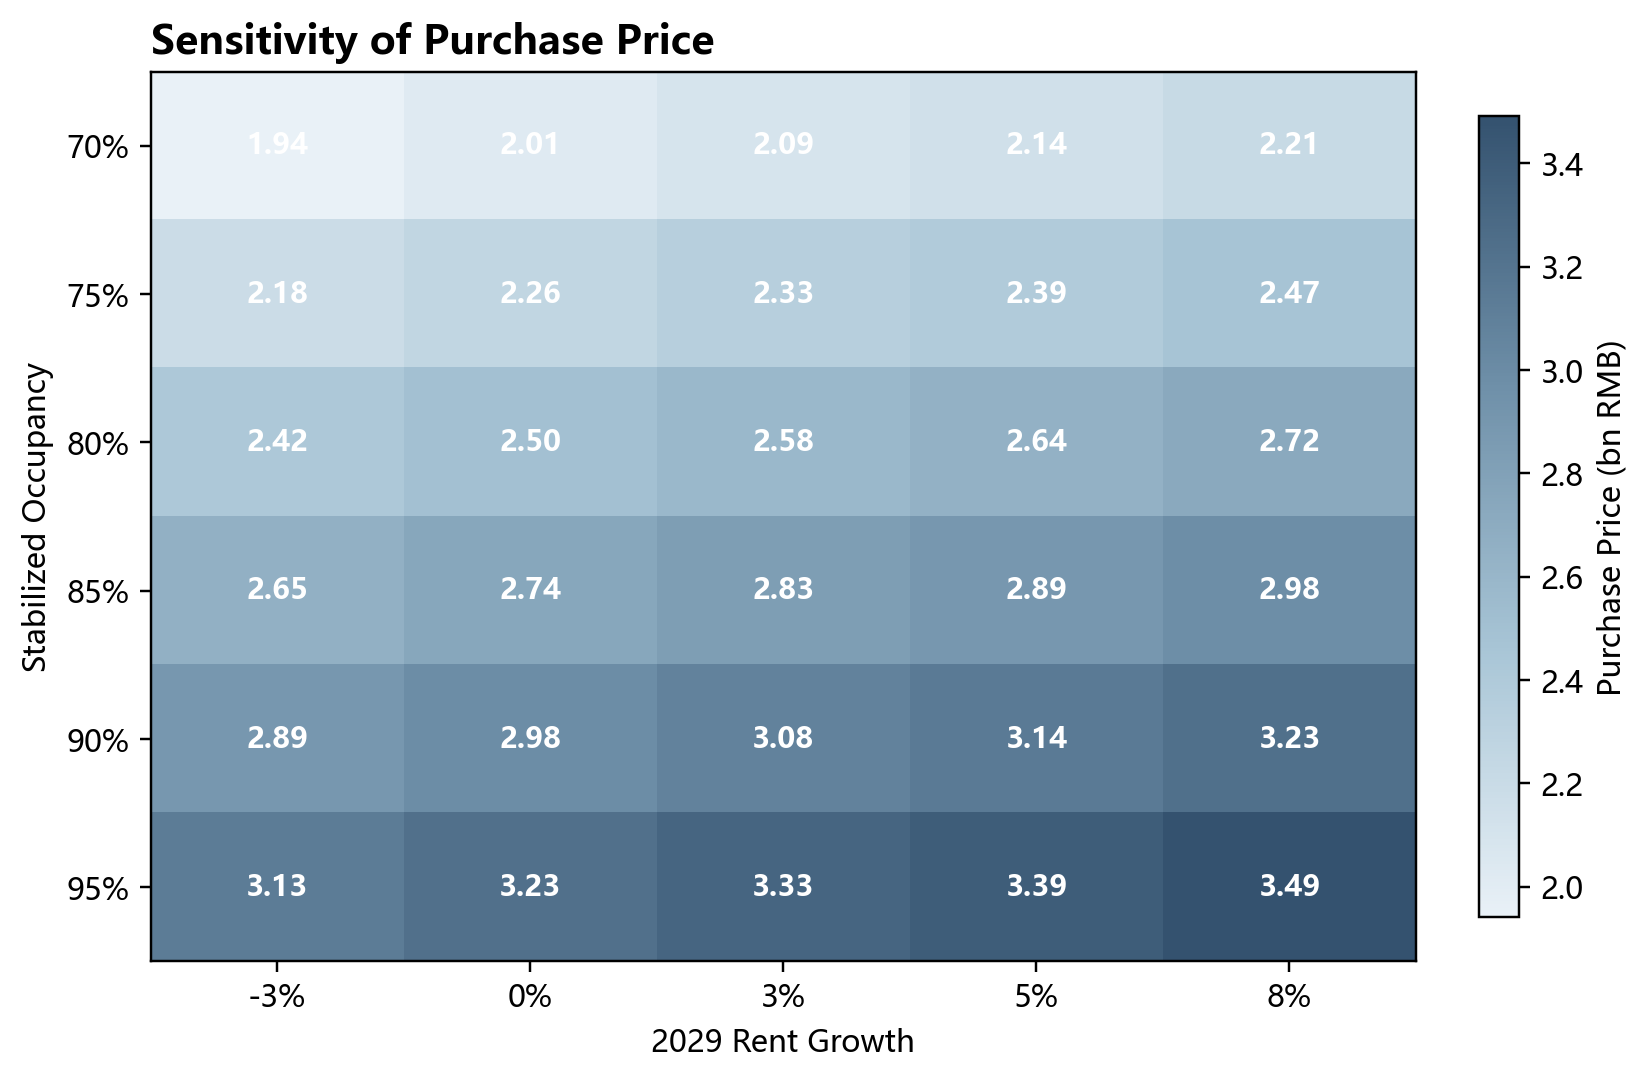
\includegraphics[width=0.88\textwidth]{figures/sensitivity_heatmap.png}
  \caption{收购价格对稳定期出租率与 2029 年租金增长率的敏感性}
\end{figure}

敏感性分析沿用 Codex 分支口径：稳定期出租率变化时，2026 年改造期出租率相应按“稳定期出租率减 15 个百分点”估算。结果表明，估值对\textbf{出租率}比对\textbf{租金增长率}更敏感。在基准增长率 \texttt{3\%} 下，稳定期出租率从 \texttt{95\%} 下调到 \texttt{90\%}，估值下降约 \textbf{2480 万元}；而在基准出租率 \texttt{95\%} 下，租金增长率从 \texttt{3\%} 降到 \texttt{0\%}，估值下降约 \textbf{990 万元}。换句话说，本项目更像是一个\textbf{招商执行型投资}，而不是简单的\textbf{租金增长型投资}。

从扩展区间看，若稳定期出租率仅为 \texttt{70\%} 且 2029 年租金增长为 \texttt{-3\%}，估值仅约 \textbf{1.94 亿元}；若稳定期出租率达到 \texttt{95\%} 且 2029 年租金增长达到 \texttt{8\%}，估值上限约为 \textbf{3.49 亿元}。因此，若卖方要价高于 \textbf{3.4 亿元}，则不仅要求稳定期出租率接近 \texttt{95\%}，还要求 2029 年租金增长明显优于基准情形，安全边际已经不足。

\section{Step 4：开放性思考}

\subsection{非财务风险与运营建议}

除财务模型外，本项目至少面临四类现实风险。第一，\textbf{招商执行风险}。项目当前处于半停业状态，原有租户水平偏低，若重组后的品牌组合不足以恢复客流，模型中的高出租率无法实现。第二，\textbf{主力店信用风险}。影院、健身、大型餐饮等主力业态虽然引流能力强，但若客流恢复慢于预期，租金拖欠与退租概率会显著上升。第三，\textbf{同业竞争与消费分流风险}。项目周边已有多个成熟居住社区和商业体，若定位不清晰，则容易陷入同质化竞争。第四，\textbf{运营爬坡风险}。地铁通车预期有利于导流，但其效果可能滞后于招商与租金兑现。

若由我负责运营与招商，我会优先构建“\textbf{社区高频消费 + 少量目的性主力店}”的组合。主力业态应优先考虑精品超市、儿童教育与亲子娱乐、连锁餐饮、生活服务及轻运动健康，而不是过度押注高票房依赖的大体量主力店。社区型购物中心的稳健性本质上来自高频到访和刚性消费；通过提升日常客流，可以同步带动餐饮、零售和停车收入，使现金流结构更加稳定。

\subsection{最终建议}

综合现金流结果、敏感性分析与运营判断，我认为本项目\textbf{可以考虑收购}，但前提是收购对价应控制在 \textbf{3.33 亿元左右或以下}，并由具备社区型商业运营经验的团队负责改造与招商。如果卖方报价显著高于该水平，则项目难以满足 \texttt{12\%} 的收益率要求，投资安全边际不足，不建议出手。

\end{document}
